\begin{figure}[p]
  \centering
  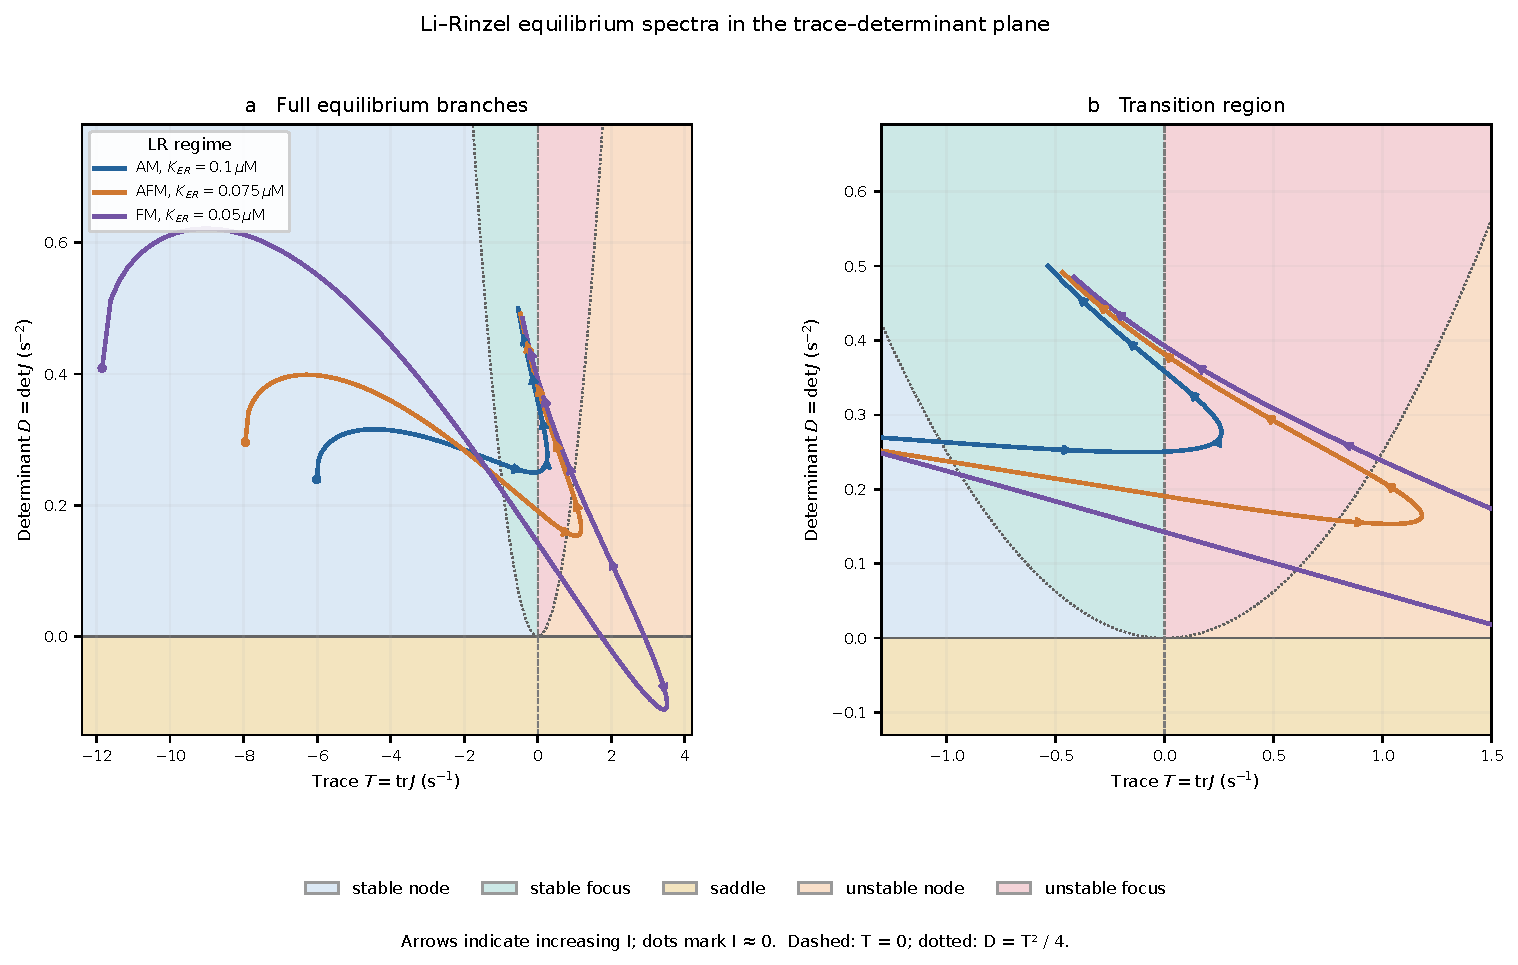
\includegraphics[width=\linewidth]{figures/figure2_lr_spectrum.pdf}
  \caption{Trace--determinant map of Li--Rinzel equilibria for AM, AFM and FM parameters. \textbf{(a)} Full computed equilibrium branches; \textbf{(b)} an enlargement of the transition region. Background colours classify the local equilibrium type. The curves are parameterized by equilibrium calcium, retaining folded branches; arrows indicate increasing $I$ and filled circles indicate the sampled point closest to $I=0$. The horizontal, vertical dashed and parabolic dotted lines are respectively $D=0$, $T=0$, and $D=T^2/4$. Spectral degeneracies on these boundaries require further conditions to establish a bifurcation.}
  \label{fig:lr-spectrum}
\end{figure}
